\documentclass[9pt,twocolumn,twoside]{../../styles/osajnl}
\usepackage{fancyvrb}
\usepackage{listings}
\journal{i524} 

\title{Charge Detection Mass Spectrometry}

\author[1,*]{Scott McClary}

\affil[1]{School of Informatics and Computing, Bloomington, IN 47408, U.S.A.}

\affil[*]{Corresponding authors: scmcclar@indiana.edu}

\dates{project-001, \today}

\ociscodes{Chemistry, Cloud, Hadoop Streaming, HPC, I524, Parallel
  Computing}
\doi{\url{https://github.com/cloudmesh/sp17-i524/blob/master/project/S17-IO-3011/report/report.pdf}}

\begin{abstract}
A Charge Detection Mass Spectrometry research application, developed
at Indiana University by the Martin F. Jarrold research group, is used
to indicate the performance and simplicity benefits of using Cloudmesh
and Ansible Galaxy to deploy and run big data software on one or more
virutal machines in the cloud. This properitery research application
was initially installed and run by hand on local servers and
Supercomputers. The Charge Detection Mass Spectrometry research
application performed well on these powerful remote systems; however,
the in-depth manual process turned out to be inefficient and too
cumbersome for the domain scientists. Therefore, Cloudmesh and Ansible
Galaxy were leveraged in order to automate the deployment of this
research application in the cloud. This modification abstracted away
the need for human interaction while maintaining an efficient,
reproducible and scalable Charge Detection Mass Spectrometry research
workflow.
\newline
\end{abstract}

\setboolean{displaycopyright}{true}

\begin{document}

\maketitle

\begin{figure}
\centering
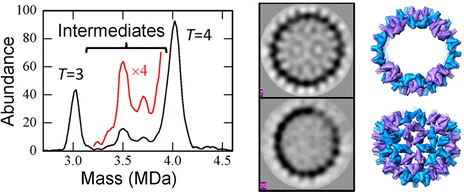
\includegraphics[height=1.35in, width=3.3in]{images/hbvassembly}
\caption{The chart to the left displays an accurate measurement of the
  Hepatitis B virus (HBV) created by the research group's Charge
  Detection Mass Spectrometry research application \cite{247}. This
  detailed mass information is used to create the images shown in the
  middle and to the right, which show 2-D and 3-D models of ions
  within the HBV.}
\label{fig:hbvassembly}
\end{figure}

\section{Introduction} \label{introduction}
\subsection{Research Background} \label{research-background}
The Martin F. Jarrold research group at Indiana University studies
Charge Detection Mass Spectrometry (CDMS). Their general day-to-day
workflow consists of conducting many scientific experiments using a
Mass Spectrometer. This expensive scientific instrument creates raw
frequency data at a rate of four (4) MB/s throughout the duration of
each experiement. The research group has developed a Fast Fourier
based application written in Fortran to processes this raw frequency
data. The Fortran application generates human interpretable output,
which assists the domain scientists in understanding the substance
analyzed in the aformentioned experiment. The outputted results
contain detailed mass information of the many ions discovered, which
is used to solve important research topics such as the measurement and
classification of the Hepatitis B virus. The mass and the abundance of
the ions discovered by the application can be plotted to determine
\emph{Intermediates} that exist between definitive peaks in the plot,
shown in Figure \ref{fig:hbvassembly}. This mass information can also
be used to generate two and three dimensional graphical
representations of the ions, which help the domains scientists
visualize the underlying structure of the Hepatitis B virus, shown in
Figure \ref{fig:hbvassembly}.

\subsection{General Problem} \label{problem}
The Martin F. Jarrold research group has the ability to generate a lot
of raw data, all of which needs to be processed by their Fortran
application, as shown in Figure \ref{fig:pipeline}. A typical day
conducting research consists of eight (8) to ten (10) one (1) hour
experiements with each experiement generating raw frequency data at a
rate of four (4) MB/s. Therefore, a single day of experiements has the
ability to generate up to 144 GB of data. The research group must be
able to process this data in a similar amount of time as the time
required to generate the raw data. If their collection of compute
resources are not powerful enough, they will quickly become inundated
with piles and piles of raw data. This day-to-day research workflow
typically strains the research group's local compute
resources. Furthermore, the research group frequently makes
algorithmic changes to the CDMS research application. When a
significant change occurs, the research group must conduct a bulk
reprocessing of months or even years worth of raw data. When a bulk
reprocess is required, the limited compute resources available to the
group becomes a significant limitation to the efficiency of their
research. Additionally, when the application is run on remote sytems,
the raw input data must be transfered to the remote systems and the
resulting output must be aggregated and then plotted in order to
visualize and interpret the results. The process of moving data around
by hand is time consuming and the process to aggregating results is
tedious.

\subsection{General Solution} \label{solution}
The research group is composed of domain scientists who do not
necessarily have backgrounds in Computer Science. Therefore, a simple
and reproducible solution must be developed to handle their day-to-day
research workflow and their bulk reprocessing requirements. The
solution to their limited compute resources consists of leveraging
multiple virtual machines in the Chameleon Cloud to conduct their CDMS
analysis. The ability to dynamically scale up or down the number of
virutal machines will align well with the evolving compute needs of
the research group. The software tools Cloudmesh and Ansible Galaxy
are at the backbone of the general solution to their
difficulties. This software provides the ability to abstract away the
technological details of the deployment and installation of virtual
machines in the Cloud as well as the explicit need to run the CDMS
application by hand. This will ensure a simple and reproducible
solution, which allows the domain scientists in the Martin F. Jarrold
research group to spend the majority of their time, effort and money
on their actual research problems and not on the technogical hurdles
of running the CDMS application.

\begin{figure}
\centering
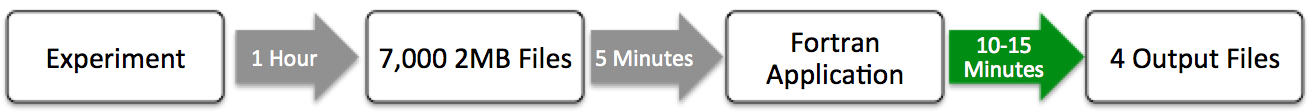
\includegraphics[height=0.45in, width=3.3in]{images/pipeline}
\caption{The Martin F. Jarrold research group currently employs the
  research pipeline shown above. This pipeline includes a one (1) hour
  experiment that creates approximately seven thousand (7,000) two (2)
  MB raw frequency files. These files need to be transfered to the
  remote compute resource(s) and processed with a Fortran application
  to generate four (4) human intrepetable output files.}
\label{fig:pipeline}
\end{figure}

\section{Execution Plan} \label{plan}
The following subsections act as a timeline regarding how the project
was divided up in order to complete all of the work by the desired
deadline. The project execution plan is simply a guide and was
followed diligently; however, some items were pushed slightly forwards
or backwards as technological challenges were faced.
\subsection{March 6, 2017 - March 12, 2017}
This week I installed Cloudmesh on my local machine, created my first
virtual machine on the Chameleon Cloud and tested Ansible Galaxy on
remote systems such as one or more Chameleon Cloud virtual machine. I
also wrote the project proposal, which eventually became this project
reoprt.
\subsection{March 13, 2017 - March 19, 2017}
This week I tested the deployment of the Intel Compiler on one or more
Chameleon Cloud virtual machine using Cloudmesh and Ansible
Galaxy. Given that I was out of town for Spring Break, I did not
expect significant progress to be made during this weeek.
\subsection{March 19, 2017 - March 26, 2017}
This week I attempted to configure the Intel Compiler to use the
Indiana University Intel license server. Using this license server
required connecting to Indiana University's Virtual Private Network
(VPN) and using Two-Step Login (Duo) from the command line.
\subsection{March 27, 2017 - April 2, 2017}
This week I deployed the Charge Detection Mass Spectrometry research
application along with the required input data on one or more
Chameleon Cloud virtual machines using Cloudmesh and Ansible Galaxy.
\subsection{April 3, 2017 - April 9, 2017}
This week I modified the source code of the OpenMP parallel Charge
Detection Mass Spectrometry research application to leverage Hadoop
Streaming.
\subsection{April 10, 2017 - April 16, 2017}
This week I benchmarked the Charge Detection Mass Spectrometry
research workflow on the Chameleon Cloud. This included varying the
number and size of the virtual machines. I also wrote Python scripts
to aggregate and plot the CDMS application's output from one or more
virtual machines and locally visualize the results.
\subsection{April 17, 2017 - April 23, 2017}
This week I ensured the reproducibility of my source code as well as
wrote and revised the final version of this report.

\section{Cloudmesh \& Ansible Galaxy} \label{ansible}
Ansible Galaxy was leveraged in order to automate the deoployment of
the required software subsystems, user code and data.

\begin{figure*}
\centering
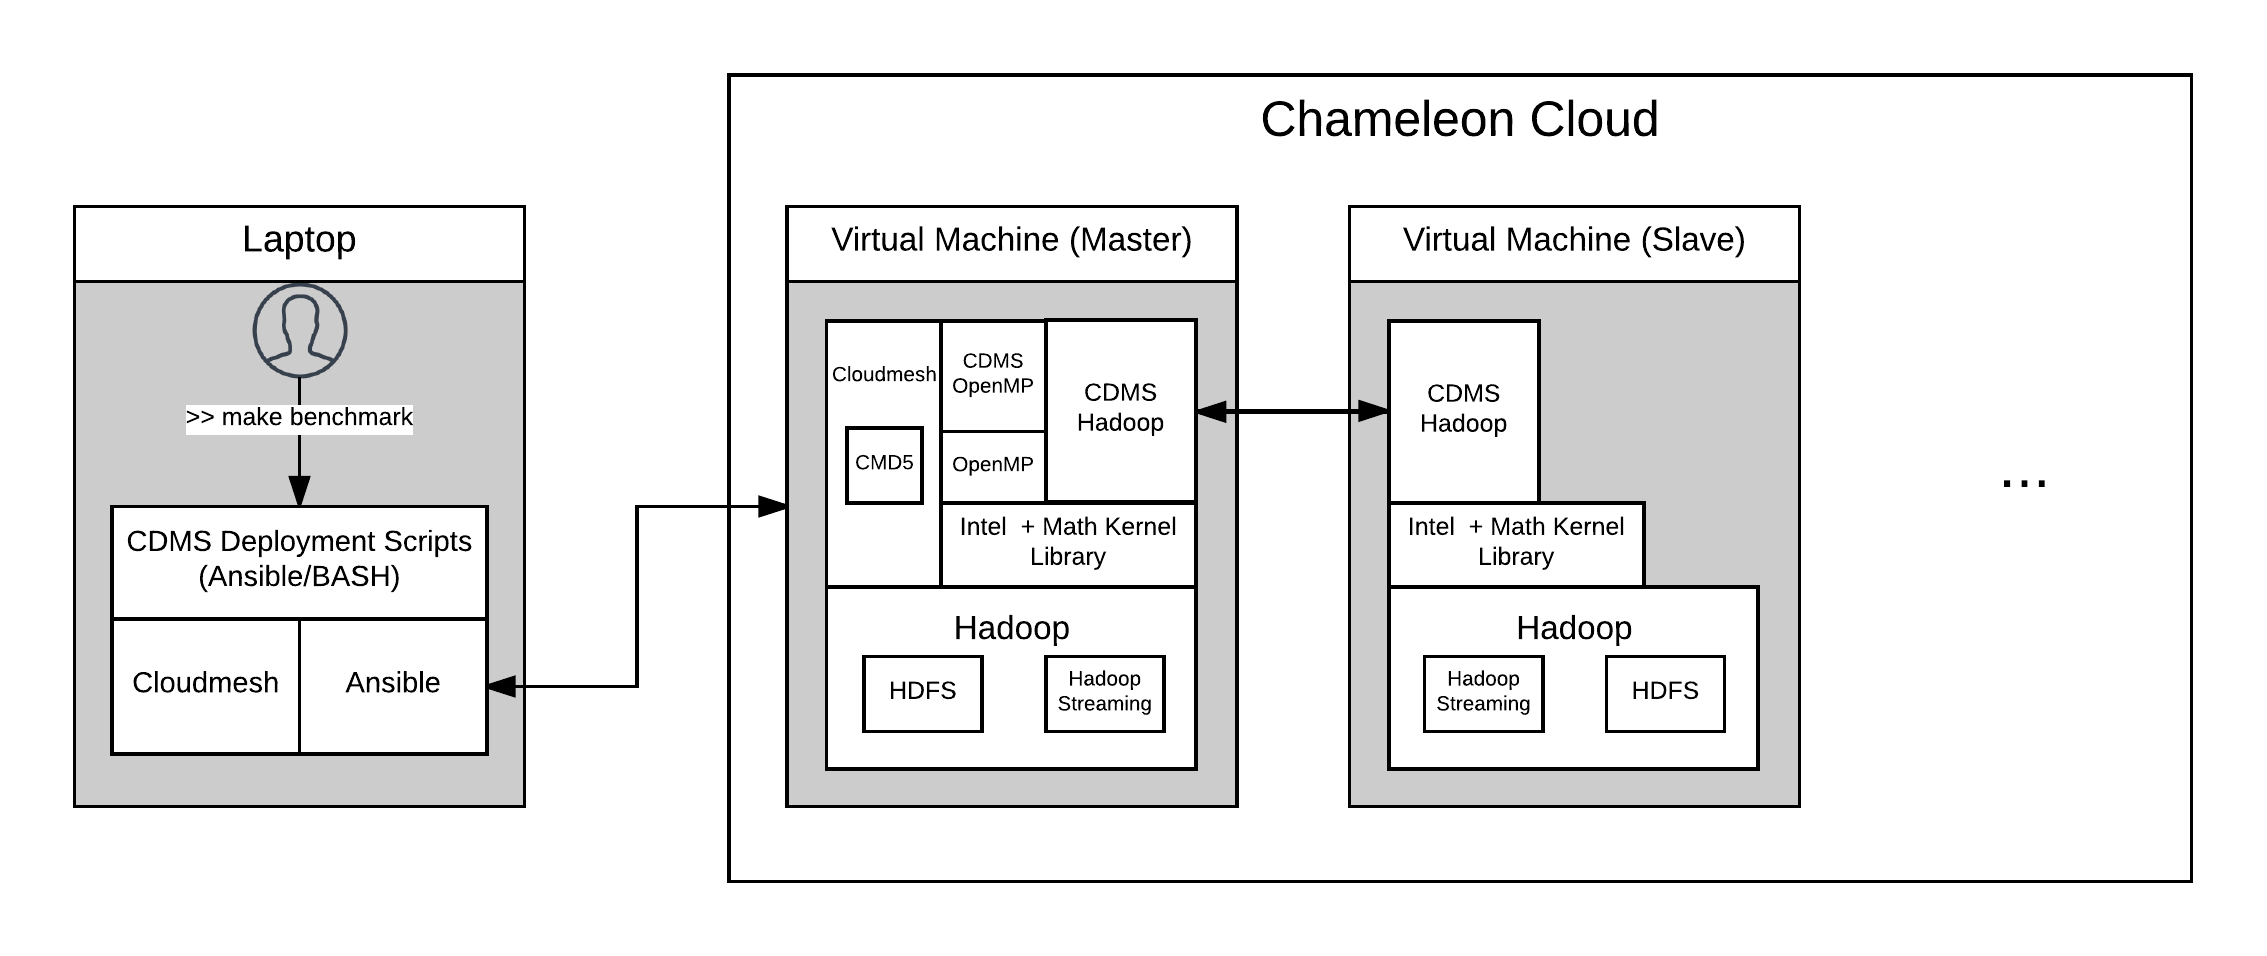
\includegraphics[height=3.0in, width=\textwidth]{images/architecture}
\caption{Architecture}
\end{figure*}

\subsection{Software Subsystems} \label{software}
The CDMS application relies on the Math Kernel Library (MKL) to
leverage efficient Fast Fourier Computations. The application also
leverages the OpenMP parallel framework in order to divide the work
amongst available CPU's. Therefore, in order to compile and run the
application, the Intel compiler is required, which provides the MKL
and OpenMP functionality.

\subsection{User Code} \label{code}
The Martin F. Jarrold Group has written a Fast Fourier Based
application written in Fortran in order to conduct their CDMS
research. This application is approximately 15,000 lines of
code. Depending on the input, about 60\% to 70\% of the compute time
is spent within external MKL libraries conducting FFT calculations.

\subsection{Data} \label{data}
The CDMS application inputs a set of raw 2 MB files. In order to
develop and test the efficiency of the deployment, a small and large
dataset was used. The small test dataset (i.e. 200 files) has a total
size of 400 MB and the large dataset (i.e. 4,506 files) has a total
size of 9.012 GB. A typical dataset for the research group is
approximately the size of the large dataset. In a single day, 7 to 10
datasets are created and need to be processed. When an algorithmic
change occurs to the research application, a large batch of archived
data requires reprocessing. In this case, terabytes of data may be
processed. This is why the parallelization and therefore the
scalability of the application is critical to the Martin F. Jarrold
research group. 

\section{Licensing} \label{licensing}
\subsection{Deployment and Benchmarking Source Code} \label{source-license}
The source code (i.e. Bash, Ansible, Python) presented is licensed
under the Apache License, Version 2.0 \cite{www-apache-lic}. 
\subsection{CDMS Source Code} \label{cdms-license}
The Martin F. Jarrold Group research group owns all of the rights to
the Fortran Source code and data. All distribution of the application
and data must be consented by the research group.
\subsection{Intel Compiler} \label{intel-license}
The Intel Compiler requires a license in order to complete the
installation. A student license is obtainable for free with an EDU
email address; however, the leveraginng the Indiana University Intel
license server would provide a more complete and reproducible
solution. In order to use the Indiana University Intel license server,
the Virtual Machines be in the Indiana University IP address
space. This can be achieved by connecting each Virtual Machine to
Indiana University's Virtual Private Network (i.e. VPN). In order to
connect to the VPN, one must connect via DUO Authentication (i.e. use
a phone or token to validate). Connecting to IU's VPN from the command
line using Ansible ended up being more of a hassle than it was
worth. 
\subsubsection{Student License Limitations} \label{student-license}
The Ansible scripts that were developed for this project leverage a
free Intel student license to compile and link the CDMS
application. While anyone can use this student license, this license
is registered to the author of this paper. This student license is
\emph{System Locked} and therefore can only be installed on at most
five (5) Virutal Machines. Once this threshold has been passed, the
Intel compiler and Intel MKL can no longer be installed. This
limitatation inhibits the reproducibility and scalability of the
research workflow. If a license registration error occurs during the
Intel build phase of the deployment of the software, please contact
the author of this paper. The author can uninstall the license from
the registered hosts, since the Intel student license is registered to
the author of this paper.

\section{Parallelization} \label{parallel}
The Charge Detection Mass Spectrometry input data is split into many
two (2) MB files. Conveniently, this data within each file is entirely
independent to the data in the other input files. Therefore, the input
data files can be processed in parallel.
\subsection{OpenMP}
The application contains OpenMP parallelization.
\subsection{Hadoop}
The source code is composed of ten thousand (10,000) lines of Fortran
code that interfaces with the Intel Math Kernel Library. In order to
use Hadoop framework, the source code would need to be rewritten in
Java. 
\subsubsection{Hadoop Streaming}
The overall structure of the input and application allowed for a
transformation of the parallelization interface from OpenMP to Hadoop
Streaming.
\begin{figure}
\centering
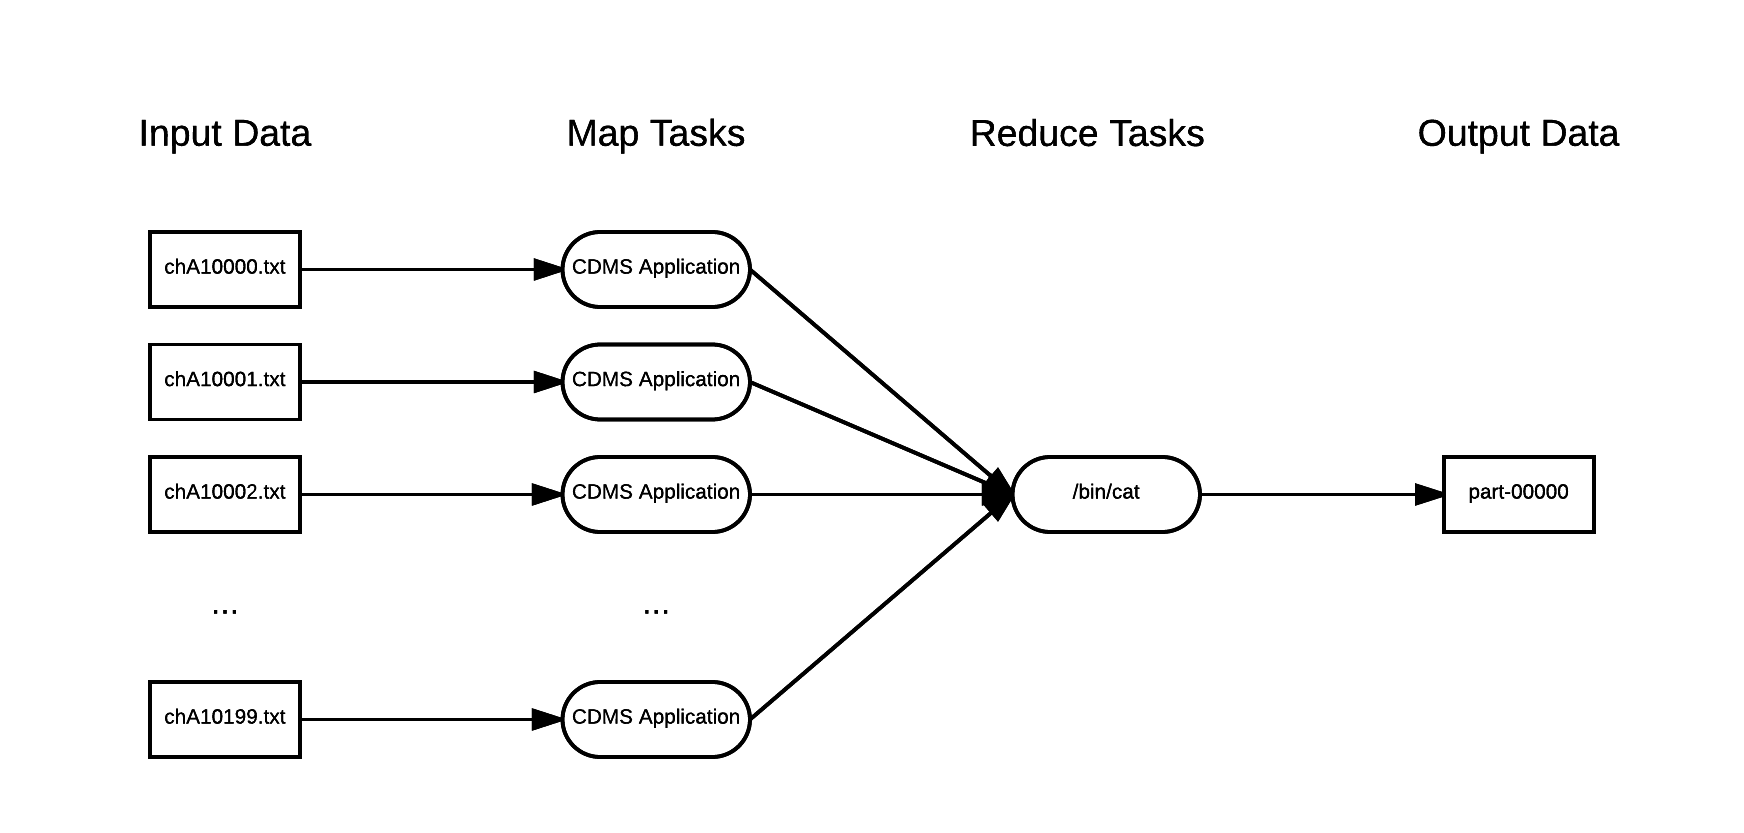
\includegraphics[height=1.65in, width=\columnwidth]{images/mapreduce}
\caption{CDMS Hadoop Streaming MapReduce}
\end{figure}

\section{Benchmark} \label{benchmark-sect}
As discussed in section \ref{code}, the application is parallelized
using OpenMP. Therefore, this application utilizes the avaialable
computational power available. Figure \ref{fig:scalability2} compares
the performance of the application on difference compute resources
(i.e. local servers, Supercomputers and clouds).

The time required to deploy and run the application in the cloud is
shown in the figure \ref{fig:benchmark}. This benchmark includes the
time required for the installation of the software subsystems as well
as the time required to run the application.
\subsection{OpenMP Scalability} \label{omp-scalability}
\begin{figure}
\centering
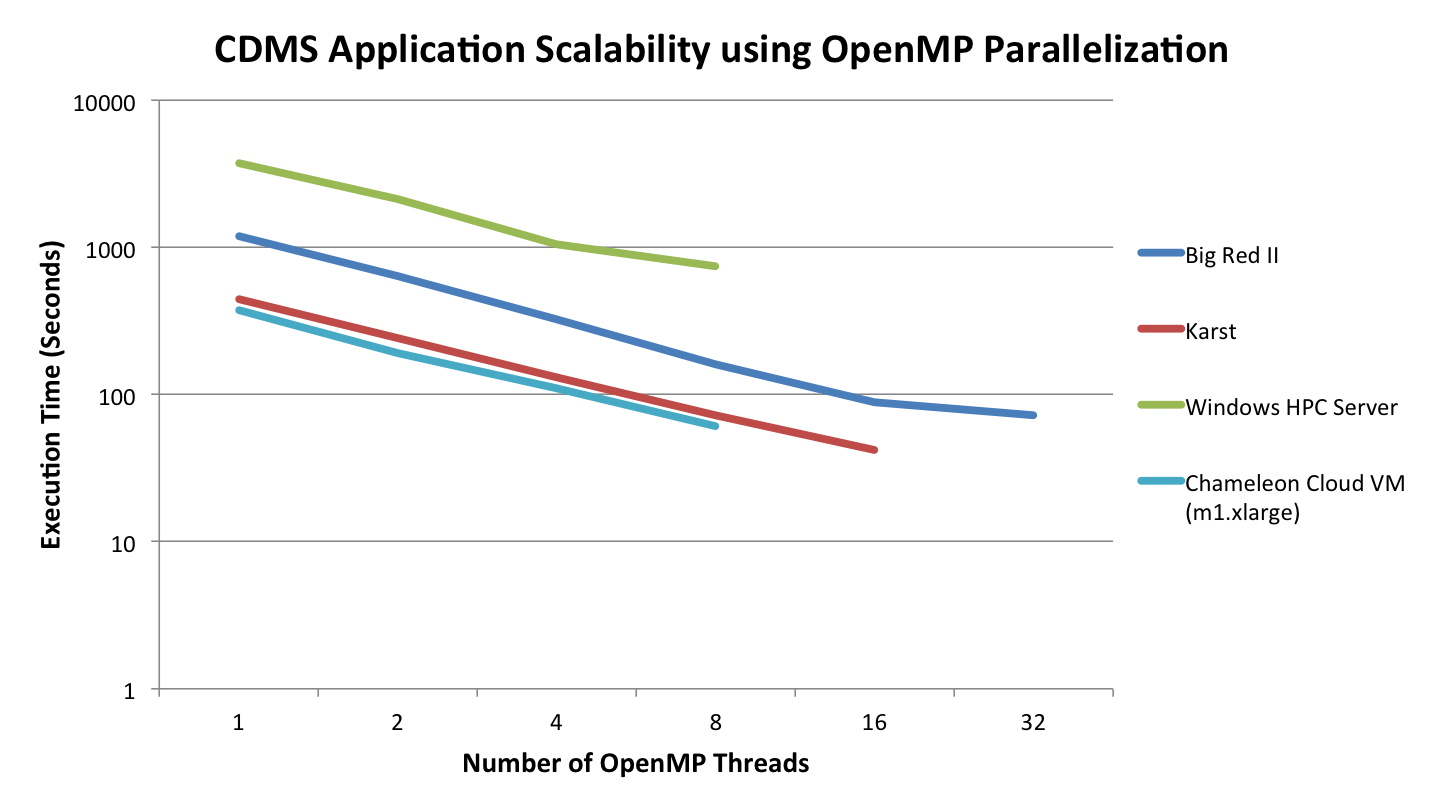
\includegraphics[height=2.1in, width=3.3in]{images/scalability2}
\caption{The figure above shows the scalability (i.e. reduction in
  time-to-solution) as the number of OpenMP threads increase on local
  servers, Supercomputers and Clouds.}
\label{fig:scalability2}
\end{figure}

\subsection{Hadoop Scalability} \label{hadoop-scalability}
The Hadoop Streaming application does not exhibit the desired
scalability. Since the application is essentially a map only Hadoop
application, the performance (i.e. total runtime) of the application
should decrease linearly with an increase in the number of nodes
deployed. However, the performance results in Table \ref{tab:hadoop}
indicate that the runtime remains relatively consistent when one (1),
two (2) or three (3) virtual machines are used to process the two
hundred (200) raw input data files. The performance analysis of the
Hadoop Streaming application will be conducted as part of the Future
Work, as explain in Section \ref{future}.

\begin{table}[htbp]
\centering
\begin{tabular}{cc}
\multicolumn{2}{c}{\bf Chameleon Cloud Virtual Machine Flavors}\\
\hline
\# Flavor & \# of vCPUs \\
\hline
m1.medium & 2 \\
m1.large & 4 \\
m1.xlarge & 8 \\
\hline
\end{tabular}
\caption{The table above indicates the number of virtual CPUs
  allocated to the various Virtual Machine flavors in the Chameleon
  Cloud. The number of vCPUs indicate the maximum degree of
  parallelism for the CDMS application.}
\label{tab:hadoop}
\end{table}

\begin{figure}
\centering
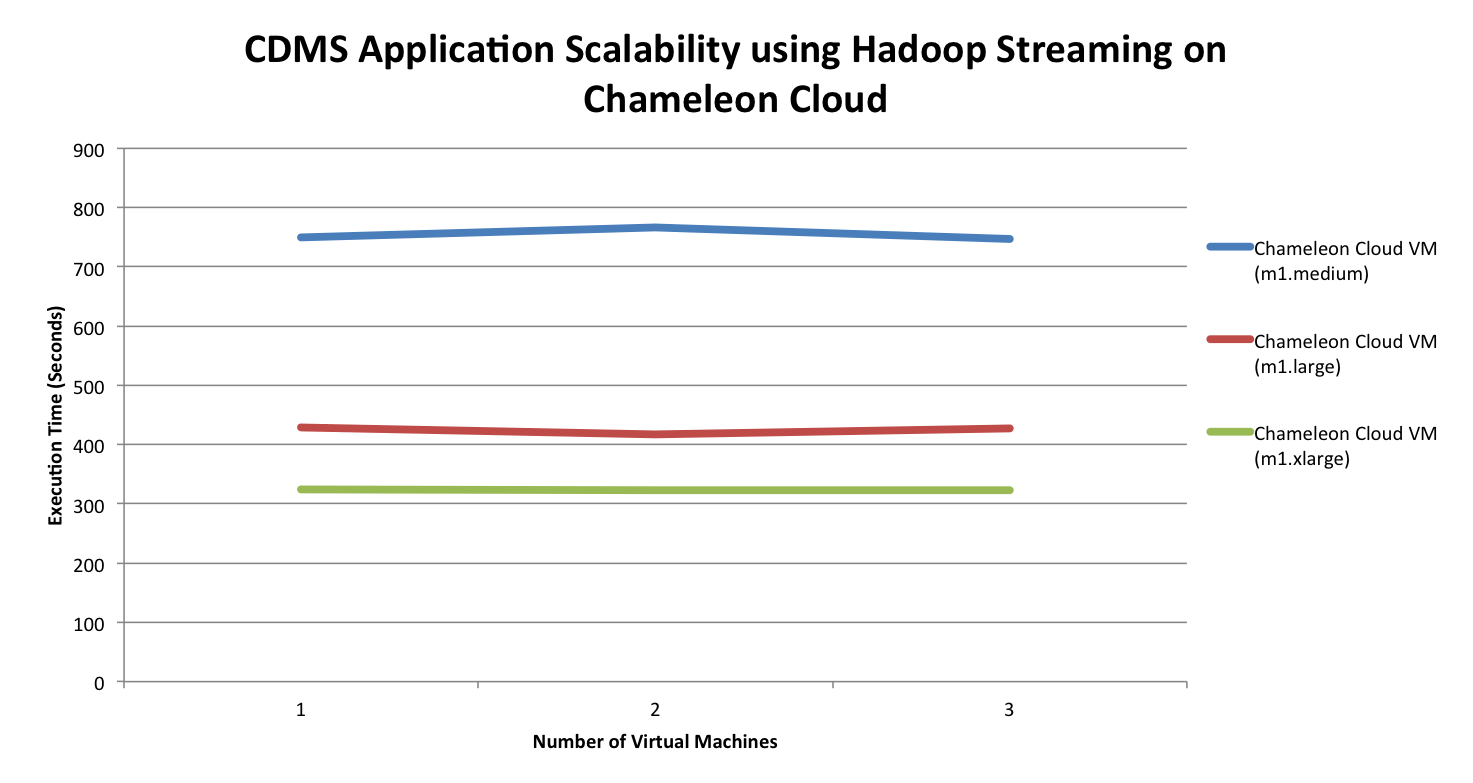
\includegraphics[height=2.1in, width=3.3in]{images/hadoop_benchmark}
\caption{The table above shows the scalability (i.e. reduction in
  time-to-solution) of the Charge Detection Mass Spectrometry Hadoop
  Streaming application as the number of Virtual Machines increase in
  the Chameleon Cloud Cluster.}
\label{fig:benchmark}
\end{figure}

\begin{figure}
\centering
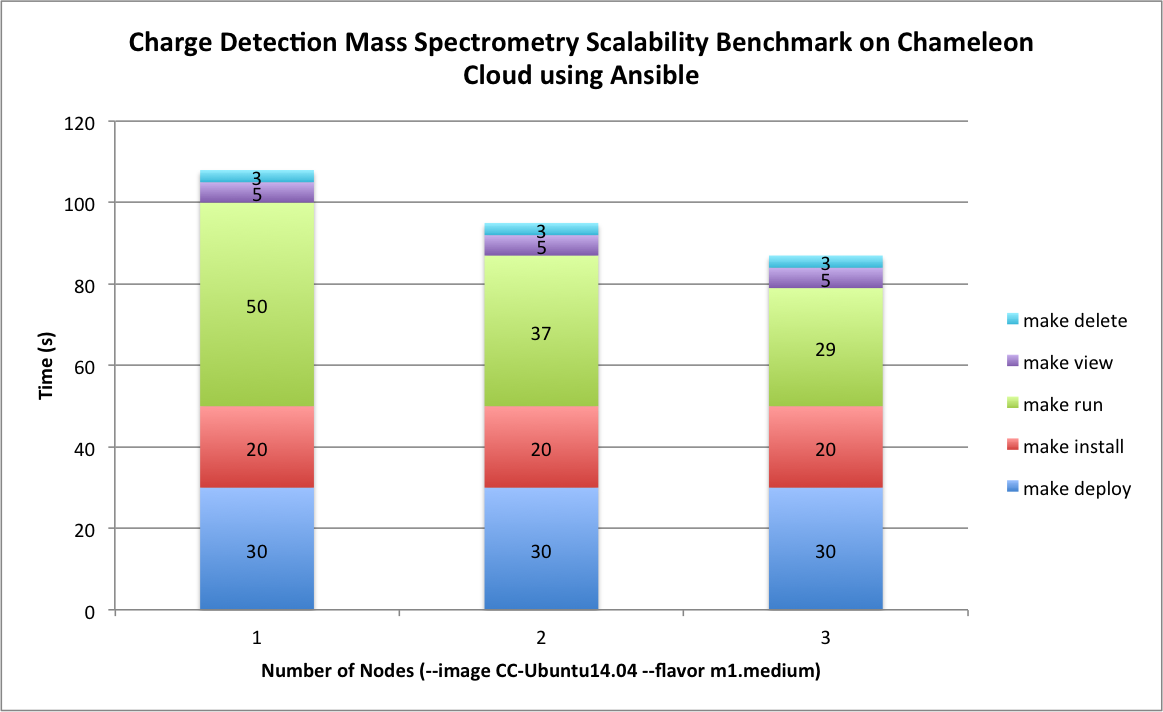
\includegraphics[height=2.1in, width=3.3in]{images/benchmark}
\caption{}
\label{fig:benchmark}
\end{figure}

\section{Reproducibility} \label{reproducibility}
This solution was specifically architected in order to be easily
reproducible. 
\subsection{Requirements} \label{req}
Must have Cloudmesh and Ansible installed locally and must have valid
$\sim$/.cloudmesh/cloudmesh.yaml file stored locally. The cloudmesh
installation is used to launch and manage VM's in the cloud. The
ansible installation is the backbone which initiates the deployment of
the cluster, installation of the required software and benchmarking of
the CDMS application.
\subsection{Fetch Code} \label{git}
The source code is hosted using Github \cite{i524-github}. This
repository contains the required Ansible and Bash scripts used to
automate the research workflow.
\noindent See the following Bash commands:
\begin{lstlisting}[language=bash]
  >> git clone [REPOSITORY]
  >> cd sp17-i524/project/S17-IO-3011/code
\end{lstlisting}
\subsection{Benchmark} \label{benchmark-info}
The benchmark discussed in Section \ref{benchmark} is available for
you to reproduce the results. A single command will deploy the Hadoop
cluster, install required software, run the three versions
(i.e. Serial, OpenMP and Hadoop) of the CDMS application, aggregate
the results, create plots of the output and delete the Hadoop
cluster. Timing information for each stage will be printed to the
screen once the benchmark has completed.
\noindent See the following Bash command:
\begin{lstlisting}[language=bash]
  >> make benchmark
\end{lstlisting}
By default the benchmark will be run on one, two and three
node(s). You can modify the maximum number of nodes (i.e. 5) to be
used in the benchmark with the following command. This will run the
benchmark with one, two, three, four and five node(s).
\noindent See the following Bash command:
\begin{lstlisting}[language=bash]
  >> make benchmark num_nodes=5
\end{lstlisting}
\subsection{Additional Commands} \label{other}
There are many pieces within the benchmark explained in Section
\ref{benchmark-info}. In case you would like to break up the benchmark
into individual pieces, there are seperate Bash commands
available. These commands will deploy the Hadoop cluster, install the
required software subsystems, run the application, view the results
and delete the Hadoop cluster.
\noindent See the following Bash commands:
\begin{lstlisting}[language=bash]
  >> make deploy [num_nodes=x]
  >> make install
  >> make run
  >> make view
  >> make delete
  >> make clean
\end{lstlisting}
\subsubsection{Deploy}
The \emph{deploy} Makefile option leverages Cloudmesh to deploy Hadoop
virutal machines in the Chameleon Cloud. The default number of virtual
machines that the \emph{deploy} option will create is three (3). The
number of virtual machines deployed can be changed by passing in
num\_nodes=x, where x is the number of virutal machines you would like
to be deployed in your cluster.
\subsubsection{Install}
The \emph{install} Makefile option installs necessary software
(i.e. Intel Compiler, Python, Pip, Cloudmesh, Git, Charge Detection
Mass Spectrometry, and etc.) on the master and slave virtual machines
of the active Chameleon Cloud cluster.
\subsubsection{Run}
The \emph{run} Makefile option runs the serial, OpenMP, and Hadoop
Streaming versions of the application on the active Chameleon Cloud
cluster using the small test dataset containing two hundred (200)
input files.
\subsubsection{View}
The \emph{view} Makefile option aggregates output data from the
virtual machines in the active Chameleon Cloud cluster, plots the data
using Python's matplotlib and transfers a few of the plots to the
local system in order to confirm the accuracy of the application.
\subsubsection{Delete}
The \emph{delete} Makefile option deletes all virtual machines
associated with your username in the Chameleon Cloud cluster.
\subsubsection{Clean}
The \emph{clean} Makefile option removes all local output files, if
they exist.

\section{Future Work} \label{future}
Future work includes analyzing the performance of the CDMS Hadoop
Streaming application to understand the poor scalability when running
on multiple nodes.  Future work on this project includes using larger
images and more virtual machines in order to increase the performance
of the Hadoop Streaming application. Future work includes figuring out
how to leverage Indiana University's Intel license server. This will
increase reproducibility by allowing the Intel Compiler and Intel MKL
to be installed on an unlimited number of virutal machines. Future
work includes dispersing the raw input data across multiple virutal
machines and running an instance of the CDMS OpenMP application on
each virutal machine and then aggregating the results. Future work
includes integrating Message Passing Interface (MPI) as the parallelel
backbone of the application rather than OpenMP. This will increase the
scalability of the application to more than a single virtual machine.

\section{Conclusion} \label{conclusion}
The development and analysis discussed above benefitted the Martin
F. Jarrold research group with respect to simplicity for the domain
scientists and with respect to the performance of the
application. Streamelining the entire workflow will inevitably result
in an increased in productivity for the research group. This may
result in an increase in grant funding and/or an increase in
publications for the Indiana University research group.

\subsection{Simplicity} \label{simplicity}
The use of Ansible Galaxy and Cloudmesh to run the Charge Detection
Mass Spectrometry application in the Cloud (e.g. Chameleon Cloud)
imporved the efficiency, reproducibility and scalability.

\subsection{Performance} \label{performance}
\subsubsection{OpenMP}
In comparison torunning on the Indiana University HPC clusters
(e.g. Karst and Big Red II), the application time-to-solution
diminished sigificantly. The most important and useful tool that was
developped as a result of this project was the automation of the
deployment of the necessary software subsystems, the application
itself, the necessary input data and aggregation/visualization of the
output. The use of Ansible Galaxy within this research workflow will
allow the Martin F. Jarrold research group to focus on the details of
their specific research rather than on the details of managing the
software subsystems, running the application and managing the
input/output data.
\subsubsection{Hadoop Streaming}
The Hadoop Streaming version of the CDMS application does not exhibit
optimal performance for the Martin F. Jarrold research group. If the
execution time reduced when more virtual machines were used, then this
version of the application would become a viable solution for the
research group's need to bulk reprocess raw input data. The Hadoop
streaming CDMS version of the application is a step in the right
direction; however, additional work must to be done to ensure
scalability across multiple virtual machines.

\section*{Acknowledgements}
The authors would like to thank the School of Informatics and
Computing for providing the Big Data Software and Projects (INFO-I524)
course \cite{www-i524}. This project would not have been possible
without the technical support \& edification from Gregor von Laszewski
and his distinguished colleagues.

 
\section*{Author Biographies}
\begingroup
\setlength\intextsep{0pt}
\begin{minipage}[t][3.2cm][t]{1.0\columnwidth} 
  \begin{wrapfigure}{L}{0.25\columnwidth}
    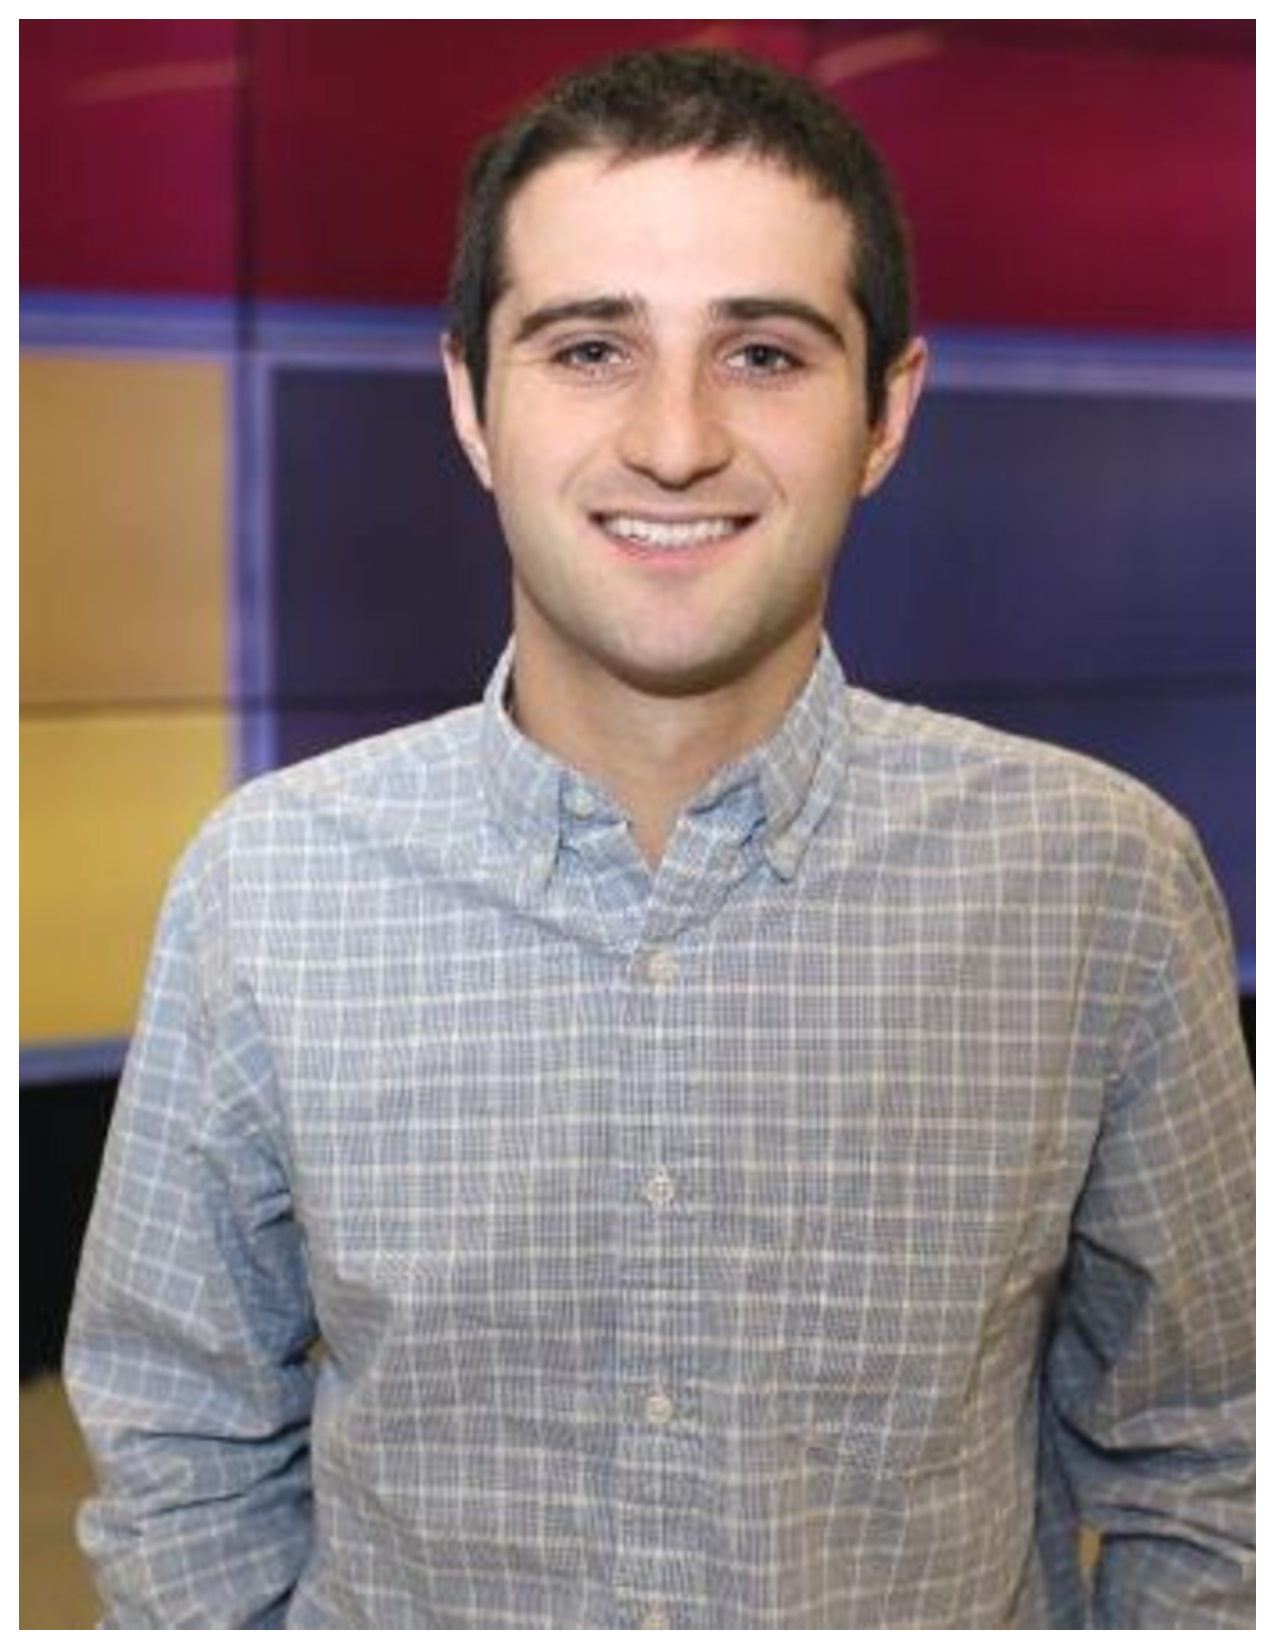
\includegraphics[width=0.25\columnwidth]{images/scott_mcclary}
  \end{wrapfigure}
  \noindent
  {\bfseries Scott McClary} received his BSc (Computer Science) and
  Minor (Mathematics) in May 2016 from Indiana University and will
  receive his MSc (Computer Science) in May 2017 from Indiana
  University. His research interests are within scientific application
  performance analysis on large-scale HPC systems. He will begin
  working as a Software Engineer with General Electric Digital in San
  Ramon, CA in July 2017.
\end{minipage}
\endgroup

\section*{} %used to create more spacing..
\section*{Work Breakdown}
The work on this project was distributed as follows between the
authors:
\begin{description}
\item[Scott McClary.] He completed all of the work for this project
  including researching, deploying, testing and benchmarking the
  Charge Detection Mass Spectrometry research application as well as
  composing this paper.
\end{description}

% Bibliography
\bibliography{references}
\end{document}

